%:= the shortest path between a commonly believed fact
%and the research question you are answering in your paper
%
%Example (Shift, CHI 2007)
%to save time for retrieving the stylus, users operate PDAs using touch
%finger tip size and occlusion make acquisition of small targets hard
% zooming does not fix that occlusion (see section “user test paper”)
% offset cursor solves the problem, but has three drawbacks
%we propose ‘Shift’. It solves the problem while avoiding the 3 drawbacks
%
%one paragraph for each logical step in that argument
%if you need more than, say, 6 paragraphs you are probably underestimating your audience and started too far back
%write in logical order, not in the chronological order in which you came up with it (this is not a diary)
%
\section{Introduction}
\ldots
\begin{figure}[h]
  \begin{center}
    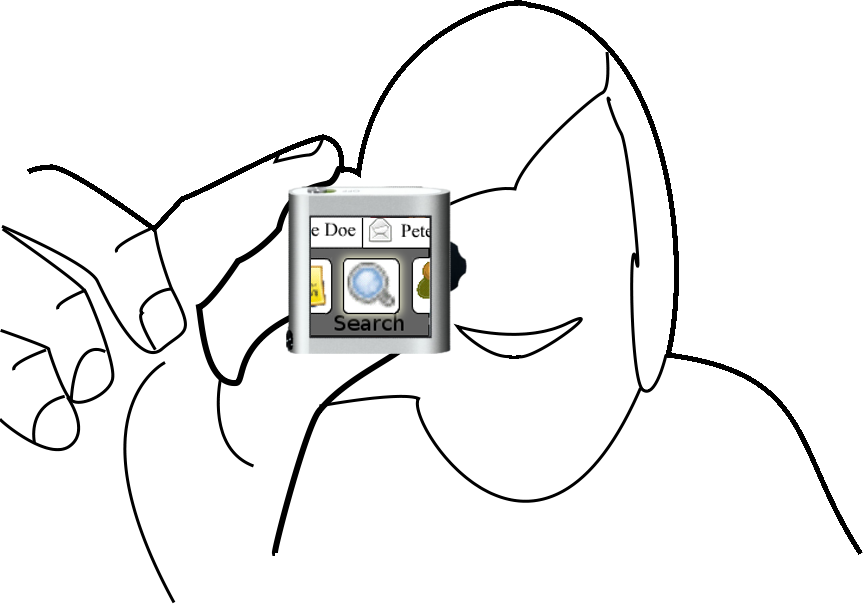
\includegraphics[width=0.8\linewidth]{imgs/main.png}
  \end{center}
  \caption{The SociaPath Device in Context}
  \label{fig:main}
\end{figure}
